\begin{itemize}
    \item Motivate the choice of parameters in~\cite{Bauer:2017ota}
    
    
    \item Vacuum stability study: fix lambda parameters to 3
    
    For extension of the Higgs sector (and in general for scalar extensions of the Standard Model) one needs to worry about 
    boundedness from below of the scalar potential, as well as absolute stability of the electroweak minimum\footnote{We remark 
    here that implications from all indirect constraints - be it flavour, electroweak precision constraints or stability 
    requirements -  should be treated as preferred parameter space in a simplified model framework. It would contradict the idea of simplified
models were these constraints taken at face value.}.  

    Regarding boundedness from below of the scalar potential in the present 2HDM + S model, we stress that provided that 
    $\lambda_{P1}, \, \lambda_{P2} > 0$ in
    %
    \begin{eqnarray}
     V_{\mathrm{P}} = \frac{1}{2} m_{P}^2 P^2 + \kappa\, (i \,P\, H_1^{\dagger}H_2 + \mathrm{h.c.}) \nonumber \\
            + \lambda_{P1} \,P^2\, \left|H_1\right|^2 + \lambda_{P2} \,P^2 \,\left|H_2\right|^2 \, ,\nonumber
    \end{eqnarray}
    %
    the study of boundedness from below at tree-level reduces to the corresponding study in the 2HDM. The boundedness from below conditions 
    in this case are well-known~\cite{Gunion:2002zf}:
    %
    \begin{equation}
    \label{stability2HDM}
     \lambda_1 > 0\,, \,\,\, \lambda_2 > 0\,, \,\,\, \lambda_3 > - \sqrt{\lambda_1 \lambda_2} \,, \,\,\, \lambda_3 + \lambda_4 - |\lambda_5| > - \sqrt{\lambda_1 \lambda_2} 
    \end{equation}
    %
    and can be inferred from analyzing the scalar potential at large field values $H_1,\,H_2 \gg v$. For $m_{H^{\pm}} = m_{H_0}$, the first two conditions 
    in~\eqref{stability2HDM} may be simply written as
    %
    \begin{equation}
     \frac{m_h^2}{v^2} (1-t_{\beta}^{2}) + \lambda_3 \, t_{\beta}^{2} > 0\,, \quad\,\, \frac{m_h^2}{v^2} (1-t_{\beta}^{-2}) + \lambda_3 \, t_{\beta}^{-2} > 0
     \end{equation}
    %
    which result in the requirement $\lambda_3 > m_h^2/v^2 = 0.258$. In figure~\ref{Fig_Stability} we show the regions of parameter space in the 
    ($m_a,\, m_{H_0}$) (left) and ($s_{\theta},\, m_a$) (right) planes for which the tree-level boundedness from below conditions~\ref{stability2HDM}
    are satisfied, assuming $m_{H^{\pm}} = m_{H_0} = m_{A_0}$.
    %
    %
    \begin{figure}[h!]
\begin{center}
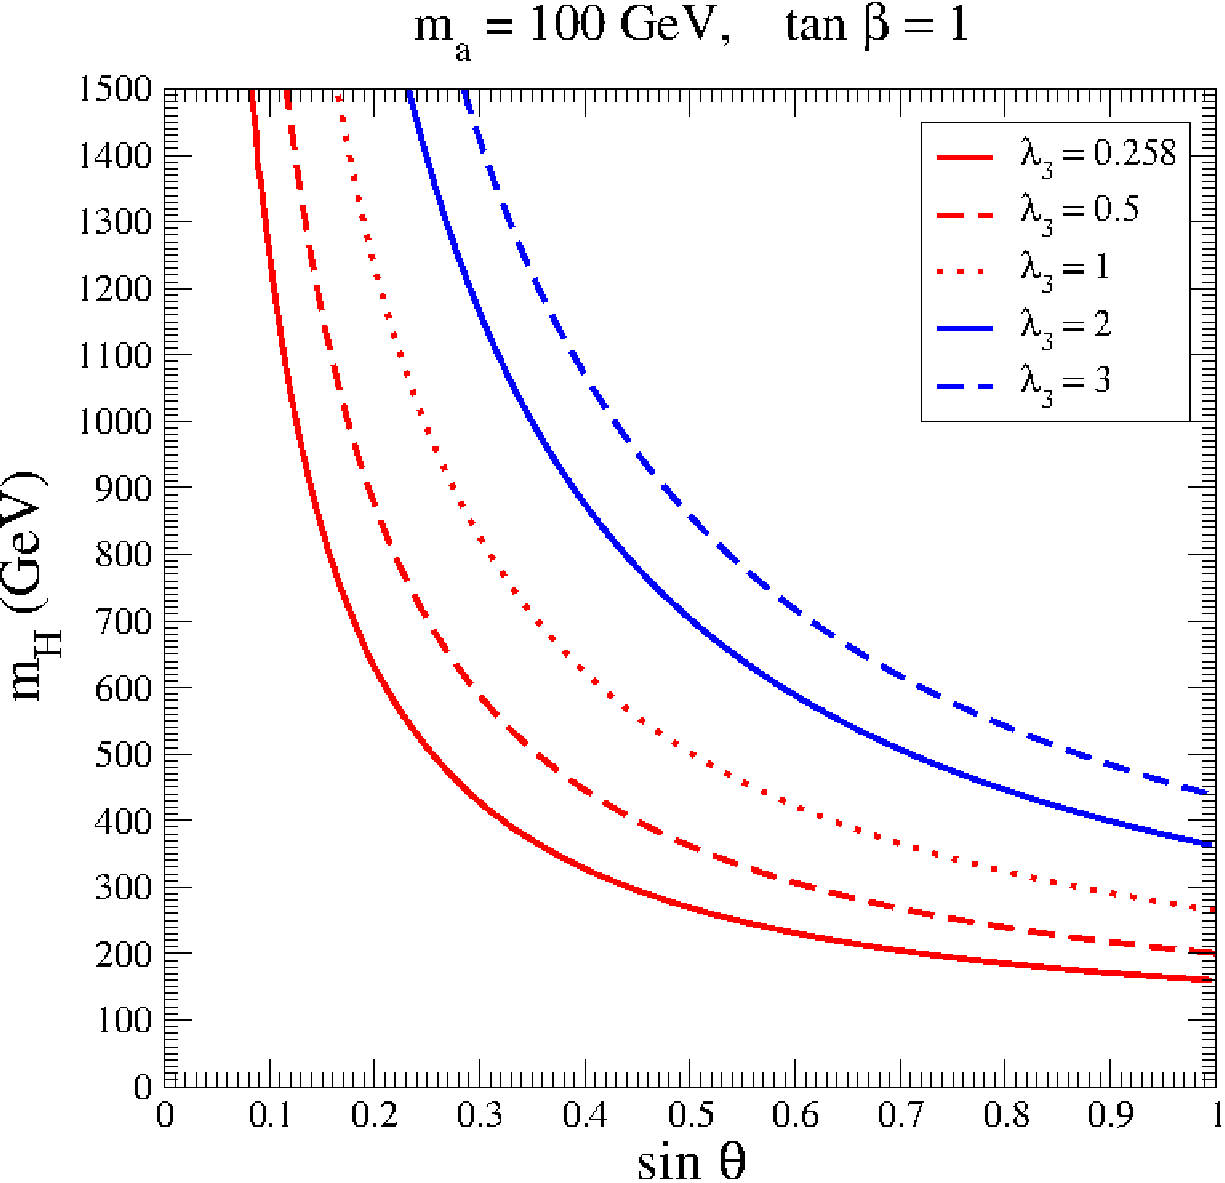
\includegraphics[width=0.485\textwidth]{texinputs/03_theoparameters/Figs/Plot_Eq.pdf}
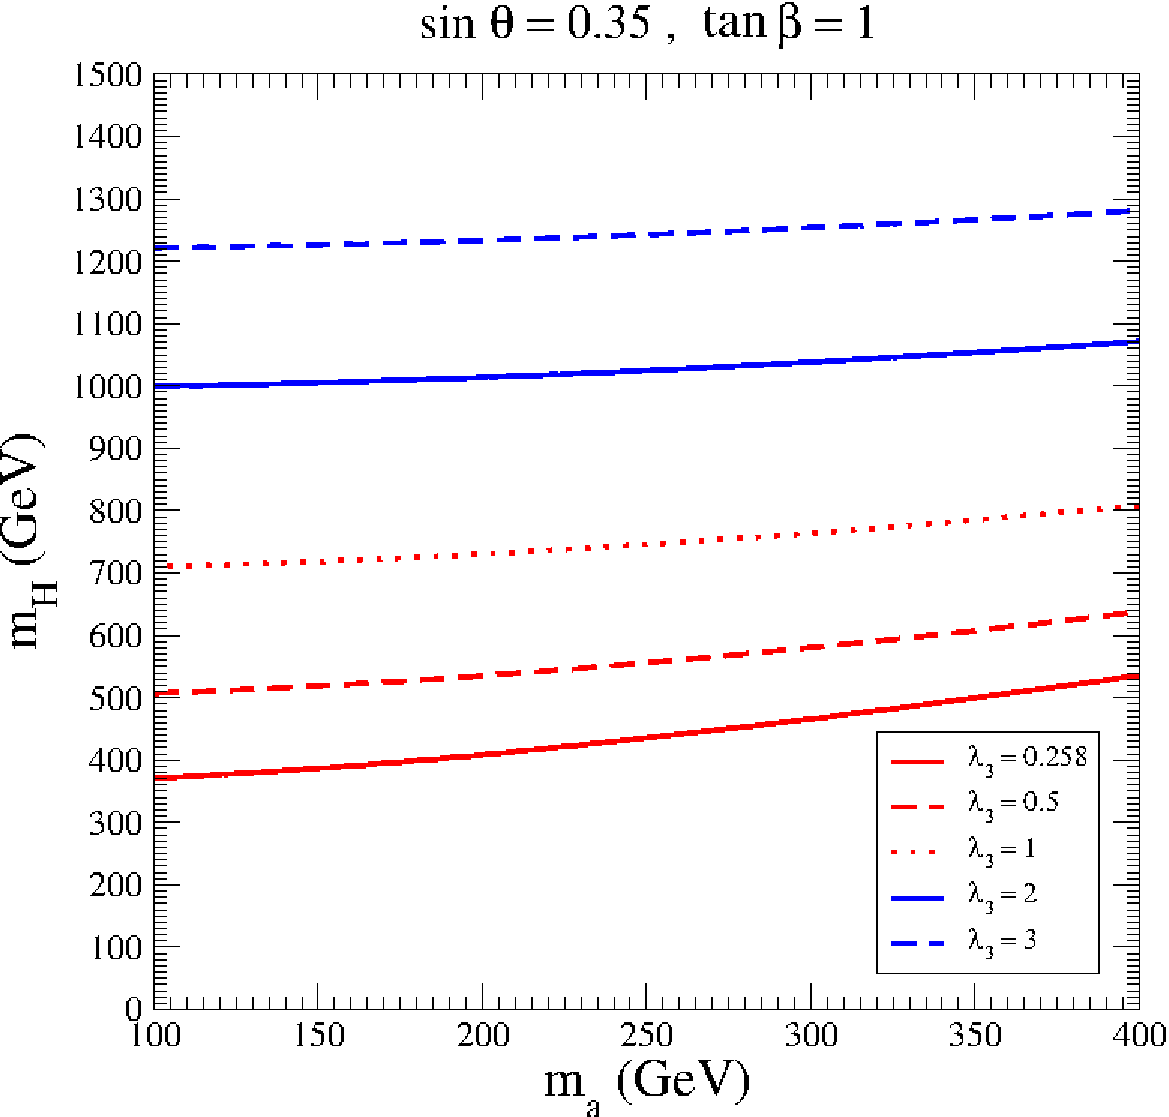
\includegraphics[width=0.485\textwidth]{texinputs/03_theoparameters/Figs/Plot_ma.pdf}
\caption{\small Regions of parameter space in the 
    ($m_a,\, m_{H_0}$) (left) and ($s_{\theta},\, m_a$) (right) planes for which the tree-level boundedness from below conditions~\ref{stability2HDM}
    are satisfied, assuming $m_{H^{\pm}} = m_{H_0} = m_{A_0}$. 
}
\label{Fig_Stability}
\end{center}

\vspace{-2mm}

\end{figure}
    %
    %
    
    Figure~\ref{Fig_Stability} shows that the region satisfying the tree-level boundedness from below conditions increases as $\lambda_3$ increases. At the same time, 
    the choice $\lambda_3 = \lambda_{P1} = \lambda_{P2}$ which we adopt in the present analysis allows the increase in $\lambda_3$  not to affect the mono-Higgs sensitivity
    via a change in the coupling $g_{aAh}$
    %
    \begin{eqnarray}
     g_{aAh} &=& \frac{c_{\theta} \,s_{\theta}}{m_{H} \,v} \left[m_h^2 + m_H^2 -m_a^2 - 2 
     (\lambda_3 - \lambda_{P1} c_{\beta}^2 - \lambda_{P2} s_{\beta}^2) v^2 \right] \nonumber \\
      &=& \frac{c_{\theta} \,s_{\theta}}{m_{H} \,v} \left[m_h^2 + m_H^2 -m_a^2 \right] 
    \end{eqnarray}
    %
    We then fix the value $\lambda_3 = 3$ as benchmark for the rest of our analysis. 
    
    \vspace{3mm}
    
    A few comments are in order. 
    
    \begin{itemize}
     \item The choice of $\lambda_3$, motivated by boundedness from below conditions, while not affecting the mono-Higgs sensitivity 
    if $\lambda_3 = \lambda_{P1} = \lambda_{P2}$, has an impact on the mono-$Z$ sensitivity since the coupling 
    %
    \begin{eqnarray}
     g_{Haa} &=& \frac{1}{m_{H} \,v} \left[ 2\, t_{2\beta}^{-1}\, s_{\theta}^2\, 
(m_h^2 - \lambda_3 v^2) + s_{2\beta}\, c_{\theta}^2 v^2 (\lambda_{P1} - \lambda_{P2}) \right] \nonumber \\
      &=& \frac{1}{m_{H} \,v} \left[ 2\, t_{2\beta}^{-1}\, s_{\theta}^2\, 
(m_h^2 - \lambda_3 v^2) \right] 
    \end{eqnarray}
    %
    does depend on $\lambda_3$ and influences the balance between $\Gamma(H_0 \to aa)$ and $\Gamma(H_0 \to Za)$ which ultimately determines the 
    $H_0 \to Za$ branching fraction. In short, the choice of $\lambda_3$, $\lambda_{P1}$, $\lambda_{P2}$ affects either mono-Higgs or mono-$Z$ sensitivities
    (or both).
    
    \item Together with boundedness from below, other potential constraints are usually considered in the context of the 2HDM and apply in general, 
    among them unitarity (see e.g.~\cite{Ginzburg:2005dt,Grinstein:2015rtl}) and absolute stability of the electroweak vacuum (see e.g.~\cite{Barroso:2013awa}). 
    In the present context we find these constraints 
    are generically weaker than the boundedness from below condition and therefore disregard them in the following. 
    
    \item The boundedness from below conditions are here evaluated at tree-level, but in a fully consistent treatment 
    they should be evaluated including the effect of radiative corrections. This is however 
    a much more involved process than what has been discussed above for the 
    tree-level case (see e.g.~\cite{Staub:2017ktc}). In addition, 
    the boundedness from below constraints discussed here are potentially sensitive to the 
    existence of UV physics which our 2HDM+S simplified does not capture, and which could modify the above picture through the presence of higher-dimensional 
    operators. Still, it is worth pointing out that for the 2HDM+S simplified model to be a good description of LHC phenomenology we require 
    the new physics scale suppressing these effective operators to be above the TeV scale (since in our scans we are considering scalar masses up to $\sim 1$ TeV), 
    and thus the presence of these high-energy operators is not expected to be of much help in case a runaway field direction exist at tree level in the 2HDM scalar 
    potential.
    \end{itemize}
    
    
    
    
\end{itemize}